\chapter{Object Detection} \label{cha:detection}
This chapter explains into the details what is the object detection task and the methods that can solve it efficiently. An overview of other methods is given, both for the not efficient one but also for problems that may look similar but are not the same. 



\section{Task definition}
Object detection, also know as \textbf{object localization}, is an evolution of the \textbf{image classification} (\Cref{fig:imgAnalysisType}). In classification, an algorithm should produce a list of all the classes of objects inside the image. Instead, the detection not only calculates which object class exist but also how many occurrences are present for each class. Then the complex part, and the most interesting one for this thesis application, is localizing where those elements are placed inside the image. The position is not considered as a point but as a bounding box defined as the smaller rectangle that contains the entire element. An example of object detection is shown in~\Cref{fig:sampleYolo}.
\begin{figure}[!h]
	\centering
	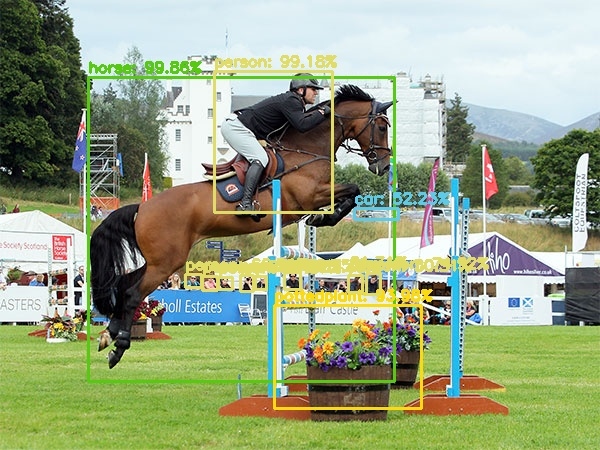
\includegraphics[width=0.8\linewidth]{images/ex1_yolo.jpg}
	\caption{Object detection applied on a sample image.}
	\label{fig:sampleYolo}
\end{figure}

\subsection{Similar tasks}
Object detection can be additionally improved to extract even more information from an image.\\
The main evolutions, shown in~\Cref{fig:imgAnalysisType} are:
\begin{itemize}
	\item \textbf{Semantic segmentation:} took all the bounding boxes produced by an object detector, and for each one, it calculates the pixels that belong to the object itself and the one that not. Doing this each class has its own colour associated. As result, the algorithm knows for each pixel if it belongs to one label (semantic division) associated with the image or to the background (yellow in the image).
	\item \textbf{Instance segmentation:} is similar to semantic segmentation, but in this case, each instance of an object is considered as a new element. In fact, the three cubes in the figure have associated different colours.\\
	This task is solved by the \textbf{Mask-R-CNN algorithm} (\Cref{sec:maskRCNN})
	\item \textbf{(Human) pose estimation:} is the more complex task between the five. Mainly applied to people, this challenge consists in the estimation of the 3D position of the body. The idea is to build up a skeleton of the person in the image and understand how its body limbs are positioned. This functionality is important to understand what a person is doing in the image.\\
	This task is solved by the \textbf{OpenPose estimation algorithm} (\Cref{sec:openPose})
\end{itemize}
\begin{figure}[!h]
	\centering
	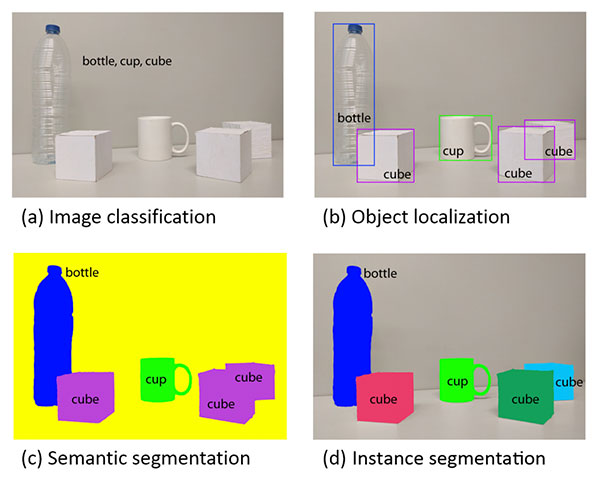
\includegraphics[width=0.7\linewidth]{images/types-of-img-analysis.jpg}
	\caption{Similar problems respect to object localization/detection.}
	\label{fig:imgAnalysisType}
\end{figure}



\section{State of the art algorithms}
Object detection has a lot of application both in real-time, such this one, but also into safety-critical scenarios like cars with autonomous driving. This division brings out two different metrics: precision and speed. The ideal detector is both fast and precise, but this algorithm does not exist yet. The methods can be divided into two.\\
The solution mainly focused on speed: YOLO (\Cref{sec:yolo}) and SSD (\Cref{sec:ssd}).\\
Instead, the one mainly focused on precision is R-CNN (\Cref{sec:r-cnn}).


\subsection{YOLO (You Only Look Once)} \label{sec:yolo}
YOLO\cite{yolo} was initially designed in 2016. At that time was the first object detector approach to use a single \textbf{CNN (Convolutional Neural Network)}. Redmon et al. goals were to create an extremely fast detector. An overview of the overall procedure is to show in~\Cref{fig:howItWorks_yolo}, and the architecture in~\Cref{fig:architecture_ssdVSyolo}.\\
The image shows a two steps procedure, but these steps are solved in parallel. This is the core idea of the paper. A single CNN can be highly optimized.\\
The YOLO procedure works as follow\footnote{The original presentation of YOLO by Redmon at the CVPR 2016 can be found \href{https://www.youtube.com/watch?v=NM6lrxy0bxs}{here}.}:
\begin{itemize}
	\item Preprocess: The image is resized to fit the standard input dimension of the CNN
	\item Left image: Then it is divided into a grid of CxC cells
	\item Top image: Each cell proposes some bounding box centred on it that can match elements in the background. To each box is associated value describing the probability that it contains one of the elements of the image.\\
	At most one detection per box can be selected as correct. This rely on the assumption that two correct bounding boxes cannot share the centre. This is both an efficient idea but also a big limitation. Too small elements, close to each other, cannot be both detected.
	\item Bottom image: To each cell is associated with a probability regarding a class that represents the class that can be found in that cell if an element exists in it.\\
	I.e. the cyan cells means: "if there is something here, it will belong to class 'DOG' ".
	\item Right image: the two partial elaborations are merged. The most likely bounding boxes are chosen and classes are associated to them according to the probability for each cell in the probability map.
\end{itemize}

That was the first YOLO version, in this thesis is used the third\cite{yoloV3}. Mainly the changes were about recognition of a wider set of classes and small implementing details to improve the overall precision of the algorithm.\\
\\
The output of the CNN is generated extremely fast and it is accurate but has a big problem. Often if two classes have similar probabilities or the shape of the element is not perfect YOLO might propose more than one bounding box for each element. That's the case of~\Cref{fig:sub_noNMS_yolo} where the truck is classified both as "truck" but also as "car". The same happens to the person that has been seen twice.\\
To solve this, it is necessary to apply a new technique: Non-Maximum Suppression

\subsubsection*{NMS (Non-Maximum Suppression)}
This technique\cite{nms} is post-processing that works on the bounding boxes proposed, as output, from YOLO or other detectors. It does not consider the source image. The goal of this procedure is to refine the bounding boxes proposed and choose which subset of them is better to fit the final image prediction. Two examples of applications are shown in~\Cref{fig:nms}\\
The main flow of the algorithm is as follow:
\begin{itemize}
	\item The input is a list of all the boxes generated for a single image. Associated to each one there is its probability.
	\item The boxes are sorted in decreasing order according to the probability associated.
	\item Then, in order, each box is accepted or rejected according to the \textbf{IoU (Intersection Over Union)}. That is the percentage of overlapping area with an already accepted box.
	\begin{itemize}
		\item If the IoU is above a certain threshold, meaning that the two boxes overlap too much the one with the lower probability is discarded.
		\item If that's not the case, the box is accepted as a new prediction.
	\end{itemize}
\end{itemize}

The input in~\Cref{fig:sub_noNMS}, is processed and only one box is accepted (\Cref{fig:sub_withNMS}) because the IoU is very high. Instead, in~\Cref{fig:sub_noNMS_yolo} two boxes are removed respectively from two other separated boxes (\Cref{fig:sub_withNMS_yolo}) because two different subjects are involved.

\begin{figure}[!h]
	\centering
	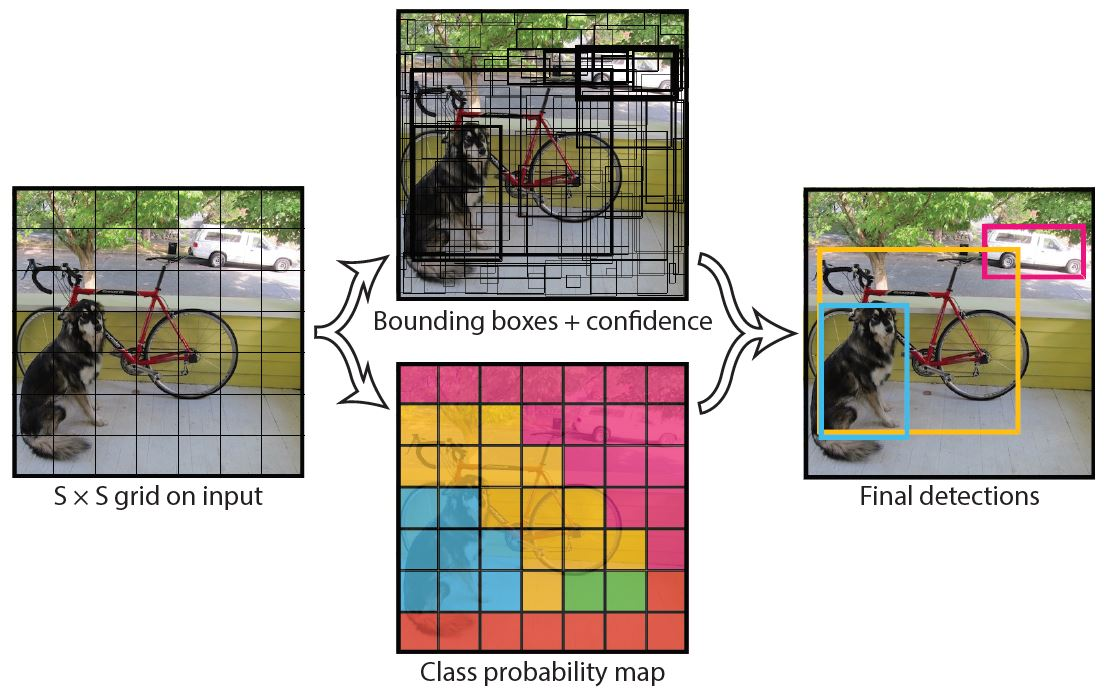
\includegraphics[width=0.8\linewidth]{images/howItWorks_yolo}
	\caption{The YOLO image elaboration based on bounding box proposal and class probability map.}
	\label{fig:howItWorks_yolo}
\end{figure}
\begin{figure}[!h]
	\centering
	\begin{subfigure}{.14\linewidth}
		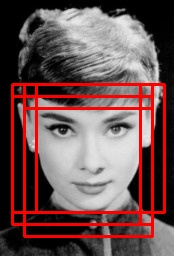
\includegraphics[width=0.9\linewidth]{images/img1_noNMS}
		\caption{Bounding boxes overlap}
		\label{fig:sub_noNMS}
	\end{subfigure}
	\begin{subfigure}{.14\linewidth}
		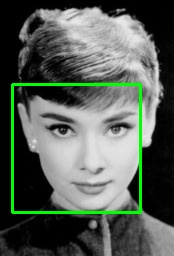
\includegraphics[width=0.9\linewidth]{images/img1_withNMS}
		\caption{Generated bounding box}
		\label{fig:sub_withNMS}
	\end{subfigure}
	\begin{subfigure}{.35\linewidth}
		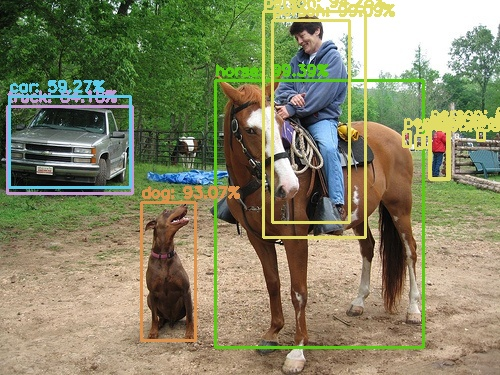
\includegraphics[width=0.9\linewidth]{images/ex2_yolo_noNMS}
		\caption{A YOLO generated bounding boxes}
		\label{fig:sub_noNMS_yolo}
	\end{subfigure}
	\begin{subfigure}{.35\linewidth}
		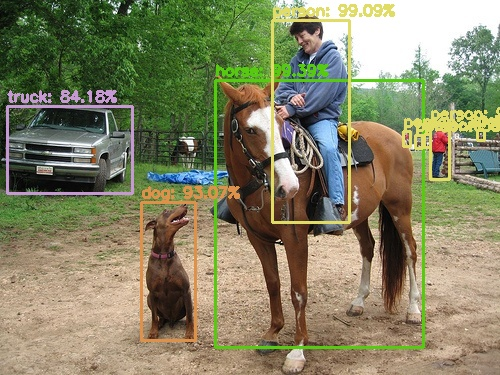
\includegraphics[width=0.9\linewidth]{images/ex2_yolo}
		\caption{Apply NMS to get correct output}
		\label{fig:sub_withNMS_yolo}
	\end{subfigure}
	\caption{Two scenarios of application of Non-maximum suppression algorithm. First: choose which of the 6 manual generated bounding boxes, on Audrey Hepburn face, should be considered the correct one. Second: refinement of the YOLO prediction output, by removing the "car" and "person" prediction.}
	\label{fig:nms}
\end{figure}


\subsection{SSD (Single Shot Multibox detector)} \label{sec:ssd}
The principal competitor of YOLO is SSD\cite{ssd}. Both are based on the same principle: use a single Convolutional Neural Network to propose bounding boxes and associate them to classes. Then optimize this CNN, as much as possible, to improve the speed performances and eventually even the accuracy.\\
The difference relies on how the two algorithms deal with the bounding boxes proposal. YOLO for each cell of the grid choose a couple of options and at most one can be chosen.\\
On the other hand, SSD works as follow (\Cref{fig:howItWorks_ssd}):
\begin{itemize}
	\item The image is divided into a grid of CxC cells, called \textbf{feature map}.
	\item Each cell can propose a set of default boxes that has a size measured in cells (i.e. 3 cells high and 2 wide).\\
	Each of these proposes comes with a confidence probability and an offset respect to the ground truth elements in the image.
	\item The process is repeated many times varying the value of C: the \textbf{granularity of the grid}.\\
	This guarantee that the algorithm is scale-independent matching both big and small subjects.\\
	In~\Cref{fig:architecture_ssdVSyolo} is shown how the convolution layers block are matched together only at the end.
	\item All the proposes are merged together to produce the final proposals.
	\item SSD internally performs NMS, to remove unnecessary detections.
\end{itemize}

\begin{figure}[!h]
\centering
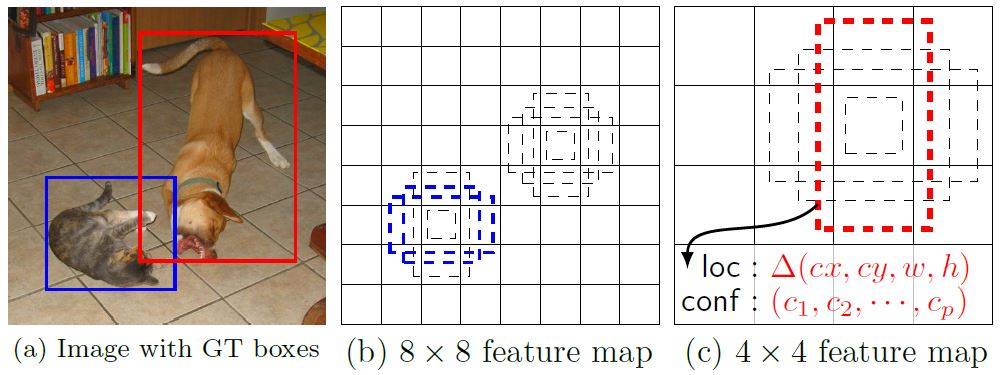
\includegraphics[width=0.8\linewidth]{images/howItWorks_ssd}
\caption{The SSD image processing and how the bounding box proposal is elaborated.}
\label{fig:howItWorks_ssd}
\end{figure}
\begin{figure}[!h]
\centering
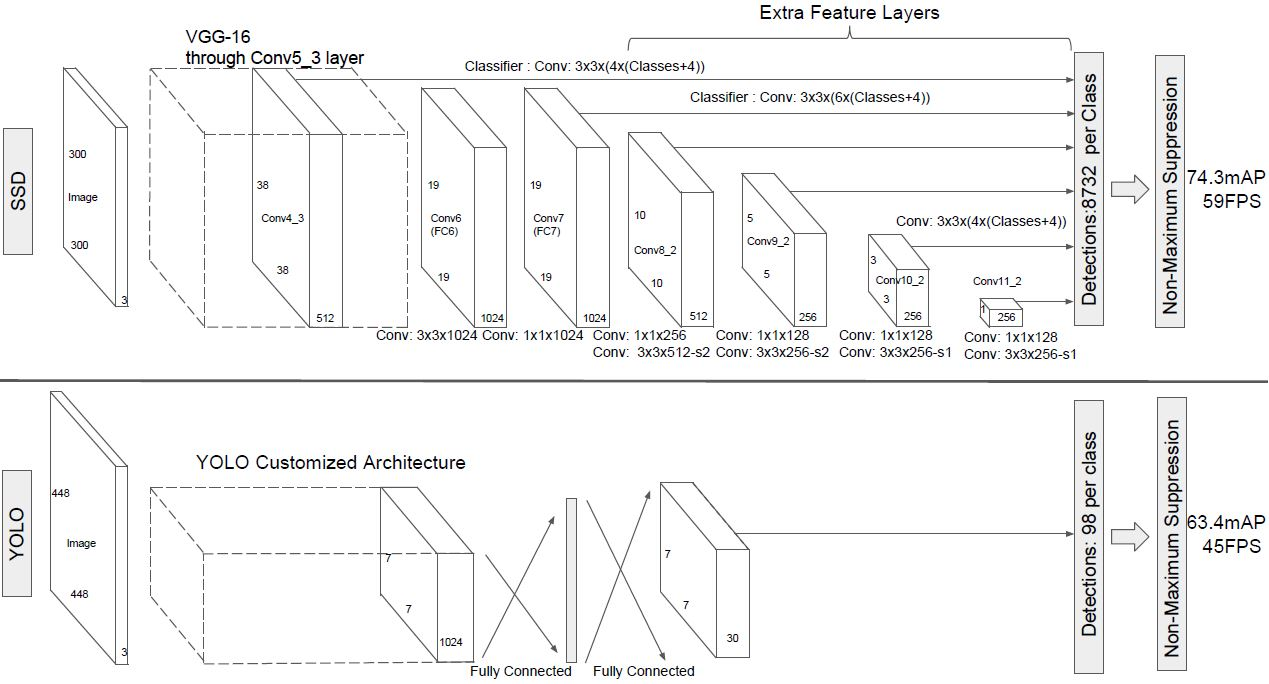
\includegraphics[width=1\linewidth]{images/architecture_ssdVSyolo}
\caption{A comparison of architectures between SSD and YOLO that is designed as a compact block. Instead, SSD is modular: divided into convolution layers of different scales, combined at the end, to make the algorithm scale-independent.}
\label{fig:architecture_ssdVSyolo}
\end{figure}


\subsubsection*{MobileNet}
The implementation of the project does not use a traditional version of SSD, but a lighter one. This model is a combination of SSD and mobileNet\cite{mobilenet} and was first proposed in that paper.\\
MobileNet is a methodology that approaches Convolutional Neural Networks to transform the architecture structure to build a much lither version of the model. The concept was first ideated to allow low power devices, such as smartphones to run computational expensive algorithms based on CNN.\\
The principle is to replace each standard convolution (\Cref{fig:sub_architecture_mobileNet1}) with a \textbf{Depthwise separable filter}. A standard convolution works on a grid of DxD pixels and for each one produce output features of depth M. This operation can be repeated N times for each source feature.\\
The operation is broken into two other simpler convolutions:
\begin{itemize}
	\item \textbf{Depthwise convolutional filters} (\Cref{fig:sub_architecture_mobileNet2}): produce only one feature output at a time, repeated M times for each DxD grid.
	\item \textbf{Pointwise convolution filters} (\Cref{fig:sub_architecture_mobileNet3}): extend the output feature of the depthwise filter to N output features.
\end{itemize}
The original paper demonstrate how these two operations stacked in a row can produce results close to the correct ones.\\
The computational cost determined by the number of parameters, used by depthwise and pointwise filters, can be further reduced by randomly remove a percentage of these parameters. According to the portion of parameters removed (25\%, 50\%, 75\%), the algorithm precision is affected.

\begin{figure}[!h]
	\centering
	\begin{subfigure}{0.32\textwidth}
		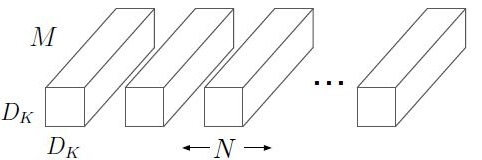
\includegraphics[width=\linewidth]{images/architecture_mobileNet1}
		\caption{Standard convolution filters}
		\label{fig:sub_architecture_mobileNet1}
	\end{subfigure}
	\begin{subfigure}{0.32\textwidth}
		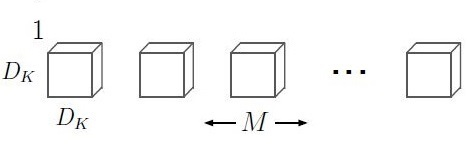
\includegraphics[width=\linewidth]{images/architecture_mobileNet2}
		\caption{Depthwise convolutional filters}
		\label{fig:sub_architecture_mobileNet2}
	\end{subfigure}
	\begin{subfigure}{0.32\textwidth}
		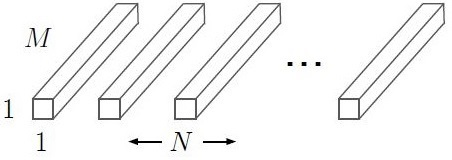
\includegraphics[width=\linewidth]{images/architecture_mobileNet3}
		\caption{1x1 convolutional filters called Pointwise convolution filters}
		\label{fig:sub_architecture_mobileNet3}
	\end{subfigure}
	\caption{The novelty of mobileNet is that it converts a traditional convolution (A), into a combination of two lighter convolutions(B-C), that produce almost the same output.}
	\label{fig:architecture_mobileNet}
\end{figure}


\subsection{R-CNN (Region-based Convolutional Neural Networks)} \label{sec:r-cnn}
\cite{r-cnn}\cite{fast-r-cnn}\cite{faster-r-cnn}\cite{mask-r-cnn}



















\section{Other famous algorithms}
\subsection{Mask R-CNN} 
\cite{mask-r-cnn}

\subsection{Open Pose} 
\cite{openpose-PAF}\cite{openpose-STAF}

\section{Which algorithm for our scenario}
better title: Algorithms performances